\tikzset{every picture/.style={line width=0.75pt}} %set default line width to 0.75pt        

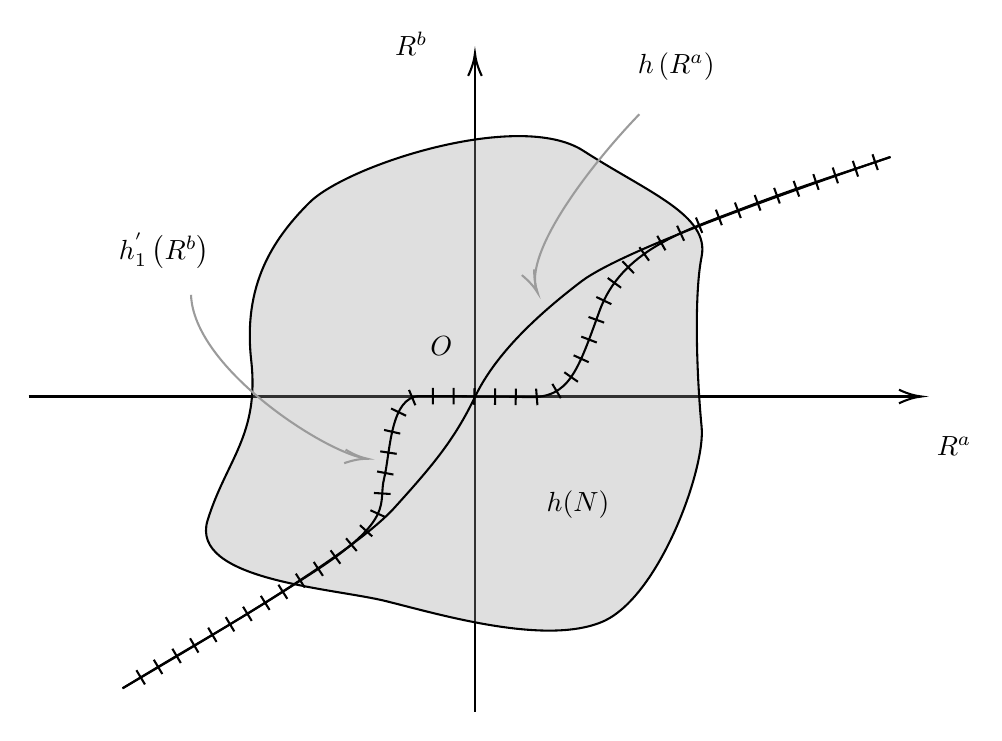
\begin{tikzpicture}[x=0.75pt,y=0.75pt,yscale=-1,xscale=1]
%uncomment if require: \path (0,724); %set diagram left start at 0, and has height of 724

%Straight Lines [id:da3129485065184029] 
\draw    (123,254.6) -- (551.2,254.6) ;
\draw [shift={(553.2,254.6)}, rotate = 180] [color={rgb, 255:red, 0; green, 0; blue, 0 }  ][line width=0.75]    (10.93,-3.29) .. controls (6.95,-1.4) and (3.31,-0.3) .. (0,0) .. controls (3.31,0.3) and (6.95,1.4) .. (10.93,3.29)   ;
%Straight Lines [id:da40717068394496947] 
\draw    (338,406.6) -- (338,91.2) ;
\draw [shift={(338,89.2)}, rotate = 90] [color={rgb, 255:red, 0; green, 0; blue, 0 }  ][line width=0.75]    (10.93,-3.29) .. controls (6.95,-1.4) and (3.31,-0.3) .. (0,0) .. controls (3.31,0.3) and (6.95,1.4) .. (10.93,3.29)   ;
%Shape: Polygon Curved [id:ds3311728239547659] 
\draw  [fill={rgb, 255:red, 155; green, 155; blue, 155 }  ,fill opacity=0.32 ] (258.2,161.2) .. controls (276.2,143.2) and (359.2,116.2) .. (390.2,136.2) .. controls (421.2,156.2) and (451.2,167.2) .. (447.2,187.2) .. controls (443.2,207.2) and (445.2,249.2) .. (447.2,269.2) .. controls (449.2,289.2) and (426.7,351.7) .. (399.2,363.2) .. controls (371.7,374.7) and (320.82,359.58) .. (295.2,353.2) .. controls (269.57,346.83) and (200.2,343.2) .. (209.2,314.2) .. controls (218.2,285.2) and (234.2,273.2) .. (230.2,237.2) .. controls (226.2,201.2) and (240.2,179.2) .. (258.2,161.2) -- cycle ;
%Curve Lines [id:da06371900121051755] 
\draw    (168.2,395.2) .. controls (219.2,365.2) and (280.2,329.2) .. (299.2,308.2) .. controls (318.2,287.2) and (328.2,275.2) .. (338.1,254.6) .. controls (348,234) and (368.2,215.2) .. (389.2,199.2) .. controls (410.2,183.2) and (500.2,152.2) .. (538.2,139.2) ;
%Curve Lines [id:da6348921142501356] 
\draw    (168.2,395.2) .. controls (209.2,370.2) and (220.2,365.2) .. (260.2,339.2) .. controls (300.2,313.2) and (291.2,306.2) .. (294.2,294.2) .. controls (297.2,282.2) and (297,254.4) .. (311.5,254.4) .. controls (326,254.4) and (332.4,254.4) .. (338.1,254.6) .. controls (343.8,254.8) and (344.4,254.4) .. (363.9,254.9) .. controls (383.4,255.4) and (387.5,242.4) .. (398,213.4) .. controls (408.5,184.4) and (438.4,174.9) .. (465.9,164.4) .. controls (493.4,153.9) and (507.9,149.4) .. (538.2,139.2)(174.88,386.47) -- (179.01,393.32)(183.27,381.43) -- (187.37,388.3)(192.21,376.12) -- (196.28,383)(200.73,371.09) -- (204.78,377.99)(209.45,365.96) -- (213.51,372.85)(217.94,360.92) -- (222.05,367.78)(226.28,355.89) -- (230.45,362.72)(234.82,350.63) -- (239.05,357.42)(243.3,345.3) -- (247.58,352.06)(251.69,339.94) -- (256.02,346.67)(260.33,334.33) -- (264.75,341)(268.44,328.71) -- (273.15,335.18)(275.89,322.92) -- (281.04,329.04)(282.59,316.59) -- (288.5,321.99)(287.62,309.4) -- (294.89,312.73)(289.34,301.08) -- (297.33,301.56)(290.86,290.72) -- (298.72,292.2)(292.36,281.03) -- (300.28,282.21)(294.21,270.71) -- (302.01,272.47)(297.6,260.38) -- (304.8,263.87)(306.23,251.42) -- (309.27,258.81)(317.69,250.4) -- (317.68,258.4)(327.75,250.42) -- (327.7,258.42)(337.8,250.59) -- (337.54,258.58)(347.68,250.64) -- (347.67,258.64)(357.73,250.76) -- (357.58,258.76)(367.46,250.82) -- (368.1,258.79)(375.29,248.54) -- (379.36,255.42)(381.05,242.92) -- (387.6,247.51)(385.53,234.75) -- (392.81,238.06)(389.22,225.75) -- (396.7,228.59)(392.71,216.27) -- (400.23,218.99)(396.48,206.66) -- (403.71,210.11)(401.95,197.5) -- (408.41,202.21)(409.03,189.42) -- (414.57,195.18)(417.21,182.65) -- (421.87,189.16)(425.83,177.19) -- (429.77,184.15)(435.39,172.31) -- (438.76,179.56)(444.47,168.37) -- (447.5,175.77)(454.09,164.59) -- (456.94,172.07)(463.24,161.13) -- (466.08,168.61)(472.77,157.53) -- (475.57,165.02)(482.14,154.08) -- (484.87,161.6)(491.55,150.73) -- (494.2,158.28)(501.01,147.46) -- (503.6,155.03)(510.37,144.29) -- (512.91,151.88)(520.04,141.06) -- (522.58,148.65)(529.53,137.89) -- (532.07,145.48) ;
%Curve Lines [id:da3876903888663663] 
\draw [color={rgb, 255:red, 155; green, 155; blue, 155 }  ,draw opacity=1 ]   (201.2,205.6) .. controls (202.36,240.13) and (263.37,280.12) .. (284.37,284.31) ;
\draw [shift={(286.2,284.6)}, rotate = 186.01] [color={rgb, 255:red, 155; green, 155; blue, 155 }  ,draw opacity=1 ][line width=0.75]    (10.93,-3.29) .. controls (6.95,-1.4) and (3.31,-0.3) .. (0,0) .. controls (3.31,0.3) and (6.95,1.4) .. (10.93,3.29)   ;
%Curve Lines [id:da04910207175146397] 
\draw [color={rgb, 255:red, 155; green, 155; blue, 155 }  ,draw opacity=1 ]   (417.2,118.6) .. controls (391.98,144.79) and (362.06,185.09) .. (367.58,203) ;
\draw [shift={(368.2,204.6)}, rotate = 244.8] [color={rgb, 255:red, 155; green, 155; blue, 155 }  ,draw opacity=1 ][line width=0.75]    (10.93,-3.29) .. controls (6.95,-1.4) and (3.31,-0.3) .. (0,0) .. controls (3.31,0.3) and (6.95,1.4) .. (10.93,3.29)   ;

% Text Node
\draw (559,272.4) node [anchor=north west][inner sep=0.75pt]    {$\mathbb{R}^{a}$};
% Text Node
\draw (298,77.4) node [anchor=north west][inner sep=0.75pt]    {$\mathbb{R}^{b}$};
% Text Node
\draw (415,87.4) node [anchor=north west][inner sep=0.75pt]    {$h\left(\mathbb{R}^{a}\right)$};
% Text Node
\draw (165,174.4) node [anchor=north west][inner sep=0.75pt]    {$h_{1}^{'}\left(\mathbb{R}^{b}\right)$};
% Text Node
\draw (315,224.4) node [anchor=north west][inner sep=0.75pt]    {$O$};
% Text Node
\draw (371,298.4) node [anchor=north west][inner sep=0.75pt]    {$h( N)$};


\end{tikzpicture}
